%================================================================%
%======  Modelo de Monografia ( UFOP - DECOM) ===================%
% Proposta de texto em conformidade com normas da ABNT ----------%
% implementadas pelo projeto abntex2, que pode ser acessado pela %
% página  http://abntex2.googlecode.com/  -----------------------%
%================================================================%
\documentclass[12pt, % tamanho da fonte
   %openright,	     % capítulos começam em página ímpar
	oneside,		  % twoside para impressão em frente e verso.  
	a4paper,			% tamanho do papel. 
	english,			% Idioma adicional para hifenização
    brazil,				% Idioma principal 
    sumario=tradicional % Comente para o sumário ser conforme a opção padrão recomendada pela ABNT NBR 6027:2012.
	]{abntex2}
	
%------------------------------------------------------------
%------------    Estrutura do texto   -----------------------      

% Pacotes Básicos:
\usepackage[T1]{fontenc}		% Seleção de códigos de fonte.
\usepackage[utf8]{inputenc}		% Codificação do documento (conversão automática dos acentos)
\usepackage{lastpage}		    % Usado pela Ficha catalográfica
\usepackage{indentfirst}		
\usepackage{color}				% Controle das cores
\usepackage{graphicx}			% Inclusão de gráficos
\usepackage{tabularx}
\usepackage{microtype} 		  	% Melhorias da justificação
\usepackage{pdfpages}           %inserir páginas em PDF
% Pacotes Extras:
\usepackage{amsmath,amsthm}     % Símbolos Matemáticos
\usepackage[portuguese, ruled, linesnumbered,commentsnumbered, algo2e, vlined, lined, boxed, algochapter]{algorithm2e} % Algoritmos 
\usepackage{hyperref}      % Criação de links.

% Escolha da formatação das referências Bibliográficas: 
\usepackage[alf,abnt-etal-list=0,abnt-etal-cite=3]{abntex2cite}	% Citações padrão ABNT  (AUTOR, ANO)
\usepackage{etoolbox}
%\usepackage[num]{abntex2cite}  % Citações numéricas (1)
%\citebrackets[] % Usar este comando para a citação numérica aparecer com [].

% Numeração das Figuras e Tabelas
\counterwithin{figure}{chapter}
\counterwithin{table}{chapter}

% Defininção de Cores:
\definecolor{blue}{RGB}{25,25,112}
\makeatletter % informações do PDF
\hypersetup{
    %pagebackref= false,
	pdftitle={\@title}, 
	pdfauthor={\@author},
    %pdfsubject={\imprimirpreambulo},
	pdfcreator={LaTeX with abnTeX2},
	pdfkeywords={abnt}{latex}{abntex}{abntex2}{trabalho acadêmico}, 
	colorlinks=true,    % false: boxed links; true: colored links
    linkcolor=blue,     % color of internal links
    citecolor=blue,     % color of links to bibliography
    filecolor=magenta, 	% color of file links
	urlcolor=blue,
	bookmarksdepth=4
}
\makeatother

% -------------------------------------------- 
% Espaçamentos entre linhas e parágrafos 
\setlength{\parindent}{1.3cm} % O tamanho do parágrafo

% Controle do espaçamento entre um parágrafo e outro:
\setlength{\parskip}{0.2cm}  % tente também \onelineskip

% Definição de ambientes matemáticos em português 
\newtheorem{teorema}{Teorema}[chapter]
\newtheorem{axioma}{Axioma}[chapter]
\newtheorem{corolario}{Corolário}[chapter]
\newtheorem{lema}{Lema}[chapter]
\newtheorem{proposicao}{Proposição}[chapter]
\newtheorem{definicao}{Definição}[chapter]
\newtheorem{exemplo}{Exemplo}[chapter]
\newtheorem{observacao}{Observação}[chapter]

% Novos Comandos
\usepackage{tgtermes}
\renewcommand{\ABNTEXchapterfont}{\rmfamily\bfseries}

% Variáveis adicionais
\providecommand{\imprimirautorcite}{}
\newcommand{\autorcite}[1]{\renewcommand{\imprimirautorcite}{#1}} 
\providecommand{\imprimirsubtitulo}{}
\newcommand{\subtitulo}[1]{\renewcommand{\imprimirsubtitulo}{#1}} 
\providecommand{\imprimirsigla}{}
\newcommand{\sigla}[1]{\renewcommand{\imprimirsigla}{#1}}
\providecommand{\imprimiruf}{}
\newcommand{\uf}[1]{\renewcommand{\imprimiruf}{#1}}
\providecommand{\imprimircurso}{}
\newcommand{\curso}[1]{\renewcommand{\imprimircurso}{#1}}
\providecommand{\imprimirinstituto}{}
\newcommand{\instituto}[1]{\renewcommand{\imprimirinstituto}{#1}}
\providecommand{\imprimirdepartamento}{}
\newcommand{\departamento}[1]{\renewcommand{\imprimirdepartamento}{#1}}
\providecommand{\imprimirano}{}
\newcommand{\ano}[1]{\renewcommand{\imprimirano}{#1}}
\providecommand{\imprimirgrau}{}
\newcommand{\grau}[1]{\renewcommand{\imprimirgrau}{#1}}
\providecommand{\imprimirexaminadorum}{}
\newcommand{\examinadorum}[1]{
    \renewcommand{\imprimirexaminadorum}{#1}}
\providecommand{\imprimirexaminadordois}{}
\newcommand{\examinadordois}[1]{
    \renewcommand{\imprimirexaminadordois}{#1}}
\providecommand{\imprimirexaminadortres}{}
\newcommand{\examinadortres}[1]{
    \renewcommand{\imprimirexaminadortres}{#1}}
\providecommand{\imprimirexaminadorquatro}{}
\newcommand{\examinadorquatro}[1]{
    \renewcommand{\imprimirexaminadorquatro}{#1}}
\providecommand{\imprimirttorientador}{}
\newcommand{\ttorientador}[1]{
    \renewcommand{\imprimirttorientador}{#1}} 
\providecommand{\imprimirttcoorientador}{}
\newcommand{\ttcoorientador}[1]{
    \renewcommand{\imprimirttcoorientador}{#1}}
\providecommand{\imprimirttexaminadorum}{}
\newcommand{\ttexaminadorum}[1]{
    \renewcommand{\imprimirttexaminadorum}{#1}}
\providecommand{\imprimirttexaminadordois}{}
\newcommand{\ttexaminadordois}[1]{\renewcommand{
        \imprimirttexaminadordois}{#1}}
\providecommand{\imprimirttexaminadortres}{}
\newcommand{\ttexaminadortres}[1]{
    \renewcommand{\imprimirttexaminadortres}{#1}}
\providecommand{\imprimirttexaminadorquatro}{}
\newcommand{\ttexaminadorquatro}[1]{
    \renewcommand{\imprimirttexaminadorquatro}{#1}}
		
%----------------------------------------------------
\renewcommand{\imprimircapa}{ % Capa 
\begin{capa}
        \begin{center}
                \begin{DoubleSpace}
                \MakeUppercase{\imprimirinstituicao } \\
                 \MakeUppercase{\imprimirinstituto } \\
                \MakeUppercase{\imprimirdepartamento} \\
                \end{DoubleSpace}
                \vspace{5cm}
				\MakeUppercase{\imprimirautor}  \\
                \imprimirorientadorRotulo ~\imprimirorientador \\
                \imprimircoorientadorRotulo ~\imprimircoorientador \\
                        				
				\vspace{5cm}
             \textbf{{\large\MakeUppercase{\imprimirtitulo}}} \\
			 \textbf{{\large \MakeUppercase{\imprimirsubtitulo}}} \\
				\vfill
        {\large{\imprimirlocal, ~\imprimiruf \\ \imprimirano  }}
        \end{center}
\end{capa}   
} % Capa



%----------------------------------------------------
\renewcommand{\imprimirfolhaderosto}{% folha de rosto
       \begin{center}
                \MakeUppercase{\imprimirinstituicao } \\
                 \MakeUppercase{\imprimirinstituto } \\
                \MakeUppercase{\imprimirdepartamento} \\
                
                \vspace{4cm}
				\MakeUppercase{\imprimirautor}  \\
				\vspace{2cm}
			    \begin{DoubleSpace}
                \MakeUppercase{\textbf{\imprimirtitulo} } \\
                \MakeUppercase{\textbf{\imprimirsubtitulo}} \\
                \end{DoubleSpace} 
      \end{center}
    \vfill 
    \begin{flushright} 
    \parbox{0.6\linewidth}{
		\imprimirtipotrabalho~ apresentada ao Curso de \imprimircurso~ da \imprimirinstituicao~ como parte dos
		requisitos necessários para a obtenção do grau de \imprimirgrau. \\ \\
		\textbf{\imprimirorientadorRotulo}~\imprimirorientador \\
		\textbf{\imprimircoorientadorRotulo}~\imprimircoorientador}
   \end{flushright} 
		\vfill
   \begin{center}
   {\large{\imprimirlocal, ~ \imprimiruf \\
   \imprimirano} }
   \end{center} }  % folha de rosto

%----------------------------------------------------


 % Estrutura do documento e pacotes usados. Outros pacotes (packages) devem ser  adicionados ao arquivo structure.tex. 

% -- Informações para Capa e Folha de Rosto: ---------------
\titulo{Avaliação de APIs de Geocodificação em Grandes Cidades Brasileiras} 
%\subtitulo{subtítulo}
\autor{Ana Luiza Almeida Soares} \autorcite{Aluno, Nome}
\local{Ouro Preto} \uf{MG}
\data{XX de mês de Ano} \ano{2023}
\orientador{Prof. Dr. Rodrigo Cesar Pedrosa Silva}  % Nome do orientador. Caso seja uma orientadora use o comando ∖orientador[Orientadora:]{Nome}
\ttorientador{Universidade Federal de Ouro Preto} % Instituição do orientador
%\coorientador{Mestre Pedro Saint Clair Garcia}   % Nome do coorientador
\ttcoorientador{Universidade Federal de Ouro Preto} % Instituição do Coorientador
\instituicao{Universidade Federal de Ouro Preto} \sigla{UFOP}
\instituto{Instituto de Ciências Exatas e Biológicas}
\departamento{Departamento de Computação}
\curso{Ciência da Computação}	
\tipotrabalho{Monografia} % Monografia (Monografia II)
\grau{Bacharel em Ciência da Computação}

%------Nomes dos membros da banca.  
\examinadorum{Prof. Dr. Membro da Banca 1}
\ttexaminadorum{Universidade Federal de ... - UFXX}
\examinadordois{Prof. Dr. Membro da Banca  2}
\ttexaminadordois{Universidade Federal de ... - UFXX}
%\examinadortres{Prof. Dr. Membro da Banca  3} 
\ttexaminadortres{Universidade Federal de ... - UFXX}
%\examinadorquatro{Prof. Dr. Membro da Banca  4}
\ttexaminadorquatro{Universidade Federal de ... - UFXX}

% ------------------------------------------------------
\makeindex      

\begin{document} % Início do documento

\frenchspacing  % Retira espaço obsoleto entre as frases.

% ----------------------------------------------------------
% -- Elementos Pré-Textuais: -------------------------------
\pagenumbering{roman}

\imprimircapa  % Capa
\imprimirfolhaderosto % Folha de rosto
%% ---------------------------------------------------------------
% ----------------  Ficha Catalográfica  -------------------------
% ---------------------------------------------------------------
% Modelo de ficha catalográfica. Você deverá substituir esta
% folha na versão final da monografia por um pdf fornecido pela 
% biblioteca. Salve o modelo oficial como ficha_catalografica.pdf
% e use o comando abaixo para inseri-lo na versão final do texto.

%\begin{fichacatalografica}
%    \includepdf{ficha_catalografica.pdf}
%\end{fichacatalografica}



%% Modelo de Como fazer a Ficha Catalográfica:

\begin{fichacatalografica}
	\sffamily
	\vspace*{\fill}					% Posição vertical
	\begin{center}					% Minipage Centralizado
	\fbox{\begin{minipage}[c][8cm]{14cm}		% Largura
	\small
	\imprimirautorcite.
	%Sobrenome, Nome do autor
	
	\hspace{0.5cm}  \\
	\imprimirtitulo  / \imprimirautor. --, \imprimirano-
	
	\hspace{0.5cm} \pageref{LastPage} p. 1 :il. (colors; grafs; tabs).\\
	
	\hspace{0.5cm} \imprimirorientadorRotulo~\imprimirorientador\\
	
	\hspace{0.5cm}
	\parbox[t]{\textwidth}{\imprimirtipotrabalho~--~\imprimirinstituicao, ~ \\
	\imprimirinstituto, ~\imprimirdepartamento,~\imprimirano.}\\
	
	\hspace{0.5cm} % Palavras-chave do trabalho
		1. Palavra-chave 1.
		2. Palavra-chave 2.
		2. Palavra-chave 3.
		3. Palavra-chave 4.
		4. Palavra-chave 5.
		I. \imprimirorientador.
		II. \imprimirinstituicao.
		III. \imprimirtitulo  			
	\end{minipage} }
	\end{center}
\end{fichacatalografica}



%\begin{errata}

\noindent AUTOR, \textbf{\imprimirtitulo} \imprimirsubtitulo. nº de páginas. \imprimirtipotrabalho - 
\imprimirdepartamento, \imprimirinstituicao, \imprimirlocal, \imprimirano.

\begin{table}[!ht]
\centering
\begin{tabular}{|c|c|c|c|} \hline
\textbf{Página} & \textbf{Linha} & \textbf{Onde se lê} & \textbf{Leia-se} \\ \hline
16 & 10 & &  \\ \hline
\end{tabular}
\end{table}


Este elemento pré-textual é opcional e deve ser inserido no texto, geralmente após o trabalho já ter sido impresso, após a folha de rosto. Deve conter a referência do trabalho e o texto da errata com a indicação da página a linha \cite{NBR14724:2011}.

\end{errata}
%% ---------------------------------------------------------------
% ----------------  Folha de aprovação  -------------------------
% ---------------------------------------------------------------
% Modelo de Folha de aprovação. Você deverá substituir esta folha na versão final da monografia por um pdf fornecido pelo colegiado do seu curso. Salve o modelo oficial como 
% folhadeaprovacao_final.pdf e use o comando abaixo para inseri-lo na versão final do texto. 
% A versão abaixo foi feita seguindo as normas ABNT NBR 14724:2011 em vigor.

%\begin{fichacatalografica}
%    \includepdf{folhadeaprovacao_final.pdf}
%\end{fichacatalografica} Esta folha será 


\begin{folhadeaprovacao}


\begin{center}
     {\large \imprimirautor}\\
       	\vspace{2cm}	
    \begin{DoubleSpace}    
    {\large \textbf{\MakeUppercase{\imprimirtitulo}}} \\
    {\large \textbf{\MakeUppercase{\imprimirsubtitulo}}}
    \end{DoubleSpace}
		\vspace{1cm}
        
\end{center}		


\begin{flushright} 
    \parbox{0.6\linewidth}{
		\imprimirtipotrabalho~ apresentada ao Curso de \imprimircurso~ da \imprimirinstituicao~ como parte dos
		requisitos necessários para a obtenção do grau em \imprimirgrau. \\}
   \end{flushright} 

\noindent Aprovada em \imprimirlocal,~ \imprimirdata. 
\begin{center}
\vfill
       \rule{10cm}{.1pt} \\
       {\imprimirorientador} \\ {\imprimirttorientador} \\
			 Orientador 
       \vfill
			 \ifdefvoid{\imprimircoorientador}{}{
       \rule{10cm}{.1pt} \\
       \imprimircoorientador \\ \imprimirttcoorientador \\ Coorientador }
			 \vfill
       \rule{10cm}{.1pt} \\
       {\imprimirexaminadorum} \\ {\imprimirttexaminadorum} \\ Examinador
        \vfill
        \ifdefvoid{\imprimirexaminadordois}{}{
        \rule{10cm}{.1pt} \\
        \imprimirexaminadordois \\ \imprimirttexaminadordois \\ Examinador}
				\vfill
        \ifdefvoid{\imprimirexaminadortres}{}{
        \rule{10cm}{.1pt} \\
        \imprimirexaminadortres \\ \imprimirttexaminadortres \\ Examinador}
				\vfill
        \ifdefvoid{\imprimirexaminadorquatro}{}{
        \rule{10cm}{.1pt} \\
        \imprimirexaminadorquatro \\ \imprimirttexaminadorquatro \\ Examinador}
\end{center}
  
\end{folhadeaprovacao}
% --- 
%\begin{dedicatoria}
   \vspace*{\fill}
   \centering
   \noindent
   \textit{ Espaço para prestar uma homenagem ou dedicar o trabalho a alguém.} 
	 \vspace*{\fill}
\end{dedicatoria}
%\begin{agradecimentos}

Espaço para agradecer às pessoas e/ou instituições que contribuíram de forma relevante à elaboração do trabalho.

\end{agradecimentos}

%\begin{epigrafe}
    \vspace*{\fill}
    
	\begin{flushright}
   Alguma citação importante para a construção do trabalho. A fonte deve ser indicada e também deve constar na lista de referências bibliográficas.
	\end{flushright}
    
\end{epigrafe}
%--------------------------------------------------------------------------
%--------------------- Resumo em Português --------------------------------
%--------------------------------------------------------------------------

\setlength{\absparsep}{18pt} % ajusta o espaçamento dos parágrafos do resumo
\begin{resumo}
  As APIs de geocodificação online desempenham um papel significativo em aplicações que requerem informações de localização. Para garantir a qualidade dessas aplicações, é essencial avaliar a precisão das APIs utilizadas. Este estudo tem como objetivo avaliar a qualidade de cinco APIs de geocodificação implementadas no TerraLAB: Google Maps, Mapbox, TomTom, Here e Open Route Service (ORS). A avaliação foi realizada com base no erro de geocodificação em comparação com uma base de dados de referência na região metropolitana de São Paulo.
  Utilizamos várias métricas para a análise comparativa, incluindo média, desvio padrão, mediana, média aparada em 5\%, taxa de resposta (proporção entre solicitações de geocodificação e respostas) e taxa de acerto (quantidade de endereços com erro menor que 150 metros). Além disso, conduzimos uma análise espacial do erro e investigamos a relação entre discrepância e erro, usando a medida de covariância. Devido a problemas na aplicação que coleta as geocodificações, esta etapa do projeto se concentrou apenas nas APIs Mapbox, TomTom e Here, resultando em um desempenho geral insatisfatório.
  A maioria das APIs apresentou uma taxa de resposta baixa, com a maior delas ficando abaixo de 90\%, o que impactou a integridade do experimento. Em relação à taxa de acerto, todas as APIs obtiveram valores considerados insatisfatórios pela nossa equipe de pesquisa. Além disso, observamos a ocorrência de erros significativos que prejudicaram a análise espacial. No que diz respeito à relação entre discrepância e erro, não pudemos identificar uma correlação forte, possivelmente devido ao número limitado de geocodificações realizadas.
  Para a próxima fase do projeto, planejamos repetir a análise com as APIs restantes para os dados de São Paulo e estender a avaliação para os dados de Belo Horizonte
  
 \vspace{\onelineskip}
 \noindent
 \textbf{Palavras-chave}: GeoAPIs. Qualidade. 

\end{resumo}

%--------------------------------------------------------------------------
%--------------------- Resumo em Inglês --------------------------------
%--------------------------------------------------------------------------
\begin{resumo}[Abstract]
 \begin{otherlanguage*}{english}
   This is the english abstract.


   \vspace{\onelineskip}
   \noindent 
   \textbf{Keywords}: Keywords1, Keywords2, Keywords3.
 \end{otherlanguage*}
\end{resumo} % (Abstract no mesmo arquivo)

% As listas abaixo são opcionais. Caso o trabalho não possua alguma(s) dela(s) basta comentar os seus respectivos comandos.

% Lista de Figuras. 
\pdfbookmark[0]{\listfigurename}{lof}
\listoffigures*   
\cleardoublepage
% lista de Tabelas
\pdfbookmark[0]{\listtablename}{lot}
\listoftables*  
\cleardoublepage
% Lista de Algoritmos
%\pdfbookmark[0]{\listalgorithmcfname}{lof}
%\listofalgorithmes   
%\cleardoublepage

% Lista de Siglas e Símbolos. Estas listas são criadas manualmente e seus arquivos estão na pasta PreTextuais.
% ---------------------------------------------------
% ------ Lista de abreviaturas e siglas -------------
% ---------------------------------------------------
\begin{siglas}
  \item[ABNT] Associação Brasileira de Normas Técnicas
  \item[DECOM] Departamento de Computação
	\item[UFOP] Universidade Federal de Ouro Preto
\end{siglas}
%% ---------------------------------------------------
% ----------- Lista de símbolos ---------------------
% ---------------------------------------------------

\begin{simbolos}
  \item[$ \Gamma $] Letra grega Gama
  \item[$ \Lambda $] Lambda
  \item[$ \zeta $] Letra grega minúscula zeta
  \item[$ \in $] Pertence
\end{simbolos}

% Sumário:
\pdfbookmark[0]{\contentsname}{toc}
\tableofcontents*
\cleardoublepage

%% ------------- Capítulos ----------------------%%
\pagenumbering{arabic} \setcounter{page}{1}
\textual 
\chapter{Introdução} \label{Introducao}
%Contextualizar o problema e motivações
% Motivação (Por quê estes problemas/perguntas são relevantes?)

\section{Endereços e Geocodificação}

\epigraph{Quase tudo o que acontece, acontece em algum lugar. Saber o local onde algo acontece pode ser fundamental.}{\cite{longley2013}}

No livro de \cite{longley2013}, os autores exploram a relação entre a humanidade e a localização. Para eles, é evidente que a maior parte das atividades humanas ocorre no planeta Terra, e, portanto, a vida está profundamente ligada à localização. Assim sendo, compreender e manipular informações geográficas é essencial para qualquer aplicação que envolva a humanidade. Além disso, os autores explicam que decisões importantes podem ter consequências geográficas. Um exemplo disso seria uma transação financeira que, em casos extremos, poderia desencadear uma crise econômica em uma região específica.

No artigo de \cite{Zamberg2009}, o autor apresenta aspectos relevantes das informações geográficas que complementam o que foi mencionado anteriormente. Segundo ele, o endereço é a principal maneira de conceitualizar a localização no mundo atual. Isso ocorre devido ao fato de os endereços serem utilizados em diversas aplicações de diferentes áreas de estudo, como na saúde \cite{AmericaJournal2001, Kypri2009, Mazumdar2008}, nas ciências sociais \cite{Chow2011}, na análise criminal ou judiciária \cite{Olligschlaeger1998}, na análise ambiental \cite{Gilboa2006}, na ciência da computação \cite{Zamberg2009}, na economia \cite{Whitsel2006} e em outros campos.

Para atingir esse objetivo, é necessário criar uma representação computacional do endereço para que as aplicações possam utilizá-la. A representação mais comum, conforme \cite{Zamberg2009}, é a utilização de coordenadas x e y em um plano, geralmente representando latitude e longitude. Esse processo de transformação em um endereço nessas coordenadas é chamado de Geocodificação ou Georreferenciamento. De acordo com \cite{Zamberg2009}, esse processo envolve três etapas:

\begin{itemize}
   \item Processamento do endereço de entrada: o endereço é lido, dividido em componentes (rua, número, bairro, etc.), padronizado e cada campo é atribuído a uma categoria; por fim, as categorias necessárias são indexadas.
   \item Busca na base de referência: com base no algoritmo escolhido, é realizada uma busca na base de referência para selecionar e classificar potenciais candidatos como resposta.
   \item Seleção do(s) candidato(s) para resposta: após a busca, a classificação gerada é analisada e os melhores candidatos são selecionados.
\end{itemize}

De acordo com \cite{longley2013}, além de representar um endereço computacionalmente, o georreferenciamento utilizando latitude e longitude oferece várias vantagens:

\begin{itemize}
   \item Precisão espacial: é capaz de indicar com alta precisão a localização de um determinado endereço.
   \item Cálculos de distância: como é um sistema espacial, permite a obtenção de distâncias e, por consequência, o cálculo de outras métricas para o endereço.
   \item Compreensão global: é um sistema usado mundialmente e, geralmente, é mais fácil de identificar e entender.
\end{itemize}

Apesar de todas as vantagens e aplicações, o processo de geocodificação pode levar a informações incorretas. No livro de \cite{longley2013}, os autores chamam essas discrepâncias de "incertezas". Para compreender o que é a incerteza, é necessário considerar outros aspectos das falhas de informação. Nesse contexto, são introduzidos os seguintes conceitos:

\begin{itemize}
   \item Erro: a diferença entre o observado e o obtido.
   \item Falta de acurácia: a diferença entre a realidade e nossa representação dela.
   \item Ambiguidade: quando mais de um valor é igualmente provável.
   \item Indefinição: a falta de informações necessárias.
\end{itemize}

Após definir esses termos, os autores definem a incerteza como: "a medida da compreensão do usuário sobre a diferença entre o conteúdo de um conjunto de dados e os fenômenos reais que os dados devem representar" \cite{longley2013}. Em outras palavras, a incerteza é uma medida que descreve o nível de compreensão do usuário em relação ao conjunto de dados obtidos e à realidade que esses dados têm a intenção de representar. A partir dessa perspectiva, a incerteza foi aceita como uma métrica apropriada para avaliar a qualidade dos Sistemas de Informação Geográfica (SIG).

\begin{figure}[ht]
   \centering
   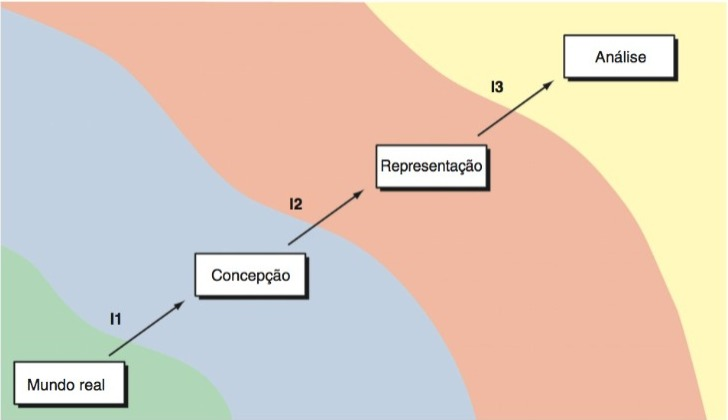
\includegraphics[width=\textwidth]{Figuras/incertezaLivro.jpeg}
   \caption{Retirada do livro \cite{longley2013}. Visão conceitual da incerteza, onde os filtros I1, I2, I3 distorcem a informação original}
   \label{fig:incerteza}
\end{figure}

\section{APIs de Geocodificação e Análise de qualidade}
% Revisão da literatura (O que já foi feito sobre o problema e o que falta fazer?)
tualmente, no TerraLAB - Laboratório de Pesquisa e Capacitação em Software \cite{terralab}, utilizamos informações geográficas para o desenvolvimento de nossas aplicações. Esses aplicativos utilizam endereços geocodificados para criar mapas, rotas, áreas de abrangência, relatar locais, divulgar eventos, entre outras funcionalidades. Isso ressalta a grande importância da geocodificação e como a qualidade desse processo impacta significativamente o que é produzido em nosso laboratório.

Para adquirir informações relacionadas a endereços, fazemos uso da geocodificação obtida por meio de APIs online de geocodificação.

Por muitos anos, a principal maneira de obter informações geográficas era através de software SIG. Conforme \cite{stein2021geoprocessamento}, um Sistema de Informação Geográfica (SIG) é um conjunto de ferramentas capazes de analisar e integrar dados geográficos, permitindo acesso fácil a dados para os usuários, sem depender de ferramentas como o GPS.

Segundo \cite{Chow2016}, embora os SIG tenham sido a ferramenta convencional por muitos anos, utilizar esse método para geocodificação requer um profissional capacitado. A ferramenta demanda o pré-processamento dos dados, criação de um localizador de endereços, customização de parâmetros, controle de qualidade e correção manual de falhas. Todo esse processo é custoso para o usuário comum. Por essa razão, a geocodificação utilizando ferramentas online retira do usuário grande parte da responsabilidade, como a manutenção da base, tornando assim o processo de obtenção de informações menos oneroso.
Apesar de a geocodificação online ser mais simples de utilizar, para que o SIG seja substituído por ela, deve-se considerar sua qualidade em relação à qualidade do SIG. No artigo \cite{Chow2016}, são avaliadas oito ferramentas de geocodificação, sendo duas delas SIGs e as demais ferramentas da internet. As ferramentas utilizadas foram: SRI ArcGIS Address Locator, CoreLogic PxPoint, Google Maps API, Yahoo! PlaceFinder, Microsoft Bing, Geocoder.us, Texas A and M University Geocoder e OpenStreetMap (OSM). Para calcular o erro, uma base de referência foi utilizada, contendo informações descritivas do endereço (rua, número, cidade etc.) e informações geográficas (latitude e longitude). Essa base é considerada a referência, pois os dados de latitude e longitude foram obtidos manualmente (por GPS ou pesquisa manual). Chamaremos essa e outras bases de referência de "base padrão ouro". A base em questão contém 940 endereços do estado do Texas, Estados Unidos da América, sendo que 78 destes são da região Central Texas, região considerada importante para o autor. O erro de cada endereço geocodificado foi calculado da seguinte forma:

\begin{align}
   \epsilon_x &= x_{\text{ref}} - x_{\text{geoc}} \\
   \epsilon_y &= y_{\text{ref}} - y_{\text{geoc}} \\
   \varepsilon_{xy} &= \sqrt{\epsilon_x^2 + \epsilon_y^2}
\end{align}

Onde:
\begin{itemize}
   \item $\epsilon_x$ é o erro da longitude,
   \item $\epsilon_y$ é o erro da latitude,
   \item $\varepsilon_{xy}$ é o erro euclidiano.
\end{itemize}
   
O estudo evidenciou que não há diferença significativa entre as ferramentas online e os SIGs. Tanto os SIGs quanto as ferramentas online apresentaram média e desvio padrão de erro semelhantes. Além disso, a taxa de resposta (ou seja, quantos endereços receberam uma resposta da ferramenta utilizada) variou entre 97,8\% e 100\%, o que é considerado satisfatório. Dessa forma, o estudo obteve êxito ao demonstrar que as ferramentas online podem ser utilizadas como substitutas dos SIGs.

Apesar de \cite{Chow2016} ter apresentado resultados significativos, o estudo apresenta algumas limitações. A principal delas é a quantidade de dados utilizada para a avaliação, além do foco restrito a uma única região (Texas, EUA). O presente trabalho busca abordar essas limitações ao conduzir a análise em uma região diferente do mundo, com ênfase no Brasil, e ampliar a quantidade de dados avaliados. Entretanto, nosso enfoque será exclusivamente em ferramentas de geocodificação online (GeoAPIs), considerando que elas já estão consolidadas no mercado e na academia.

PAREI A REVISÃO AQUI

Outro estudo importante é \cite{Clodoveu2011} que faz uma avaliação da qualidade da geocodificação do Google Maps API fornecida pelo Google Cloud Plataform \cite{GCP}. Nesse estudo, os autores utilizam uma base padrão ouro com os dados de Belo Horizonte, cidade de Minas Gerais, estado do Brasil para essa avaliação. A base conta com mais de 540 mil endereços da cidade e é mantida pela empresa de informática e informação do município de Belo Horizonte - Prodabel \cite{Prodabel}. A empresa atualiza os dados mensalmente
e tem parceria com outras 26 empresas para manter a base o mais correta possível. Ela conta com informações descritivas, sociais e espaciais do endereço. Para medir o erro, foi calculada a distância euclidiana dos pontos geocodificados para os pontos originais. A partir do erro, o estudo faz análises espacias do erro e também relaciona a acurácia descrita pela API com o erro gerado. O estudo mostrou que o Google Maps API tem taxa de acerto de 74,7\%, considerando que acertou se o erro for menor de 150 metros. Outra descoberta foi que o erro é menor nas áreas centrais da cidade, e maior na periferias. Os autores também tentaram fazer uma relação entre erro e renda, porém não foi possível vizualizar nenhuma relação direta. 

Apesar de descobertas importantes, o estudo é limitado na medida que só analisa uma API de geocodificação. Além de analisar apenas uma cidade brasileira, o que impossibilita a generalização dos resultados. O trabalho pretende trabalhar nessas limitações fazendo a análise de uma amostra da mesma base de dados, porém com outras APIs de geodificação. Além disso, iremos fazer uma análise com uma base da região metropolitana de São Paulo. O que traz uma diversidade para nosso estudo. 

\section{Objetivos}
% Objetivo (O que você pretente atingir?)
% Objetivos específicos (objetivos intermediários) 
O principal objetivo deste trabalho é avaliar o erro, a discrepância e a acurácia de cinco APIs utilizadas no laboratório de pesquisa e capacitação em desenvolvimento de software - TerraLAB. As APIs em análise são: Google Maps, TomTom, Open Route Service (ORS), Mapbox e Here. O erro será analisado quanto às respostas fornecidas pelas APIs diferirem do esperado. A discrepância medirá o nível de discordância entre as APIs. Por fim, a acurácia será utilizada para verificar a precisão das respostas fornecidas pelas APIs.

Uma parte essencial do trabalho é compreender os pontos onde essas APIs apresentam falhas, e, portanto, a análise espacial dessas medidas terá grande destaque na pesquisa.

Com isso, gostaríamos de responder as seguintes perguntas:
\begin{itemize}
   \item Qual API das utilizadas erra mais?
   \item Existe algum padrão espacial no erro?
   \item Alguma medida de variância entre as APIs (discrepância) representa o erro? 
\end{itemize}

Para chegar a essas  respostas temos alguns objetivos específicos que devem ser atendidos:
\begin{itemize}
   \item Coletar bases de dados padrão ouro;
   \item Calcular as medidas para avaliação;
   \item Avaliar as distribuição das medidas; 
   \item Correlacionar as medidas; 
   \item Avaliar de que forma o espaço se relaciona com essas medidas.
\end{itemize}





\section{Organização do Trabalho}

Um parágrafo fazendo uma descrição dos capítulos restantes do documento. 

\subsection{Estrutura da Monografia}

Segue uma \textbf{sugestão} para a estrutura da monografia: 

\begin{description}
   \item[Capítulo 1:] Introdução.
   \item[Capítulo \ref{RevisaoBibliografica}:] Revisão Bibliográfica/ Embasamento Teórico (com o referencial teórico e trabalhos relacionados).
   \item[Capítulo \ref{desenvolvimento}:] Metodologia ou Desenvolvimento (material e métodos).
   \item[Capítulo \ref{resultado}:] Resultados e Discussões.
   \item[Capítulo \ref{conclusao}:] Conclusão (e trabalhos futuros).
\end{description}


 










%\chapter{Revisão Bibliográfica} \label{RevisaoBibliografica}

Este capítulo deve apresentar uma contextualização da sua pesquisa com um resumo das discussões já feitas por outros autores sobre o assunto abordado e os conceitos principais relativos ao tema. O nome deste capítulo  de \textbf{Revisão Bibliográfica} ou \textbf{Embasamento Teórico} deve ser acordado com seu orientador.

A revisão bibliográfica é a base que sustenta qualquer pesquisa científica e  é indispensável para a delimitação do problema em um projeto de pesquisa,  para obter uma ideia precisa sobre o estado atual dos conhecimentos sobre um tema, sobre suas lacunas e sobre a contribuição da investigação para o desenvolvimento do conhecimento \cite{marconi2003}. 

Para a escrita deste capítulo, as citações e referências devem estar de acordo com a norma \cite{NBR6023:2002}, que destina-se a orientar a preparação e compilação das  referências bibliográficas de todo o documento.

\section{Trabalhos Relacionados}

Descreva os principais trabalhos realizados por outros autores sobre a temática escolhida para ser desenvolvida, apresentando os conceitos mais importantes, justificativas e características sobre o tema, do ponto de vista da análise feita pelos autores. 

É importante destacar, no contexto da pesquisa, quais os resultados já alcançados e os respectivos responsáveis e se possível uma análise  dos trabalhos consultados. Finalize a seção comparando a sua proposta de pesquisa com os trabalhos citados, destacando as semelhanças (caso existam) e a sua contribuição (o que pretende desenvolver).


\section{Geocodificação}

\section{Qualidade de dados}

\section{Erro, Acurácia e Discrepância}

\section{APIs de Geocodificação}




\chapter{Bases de Dados e Métodos de Geocodificação e Avaliação} \label{desenvolvimento}


Para avaliar a qualidade das APIs de geocodificação utilizadas no TerraLAB duas bases de dados padrão ouro foram usadas como referência. Chamaremos essas bases de Bases Gold. Com as bases, foi obtida a medida de erro e realizadas métricas diversas utilizando essa medida.


\section{Bases de Dados}
Foram coletadas duas bases de dados distintas para o presente trabalho.

A primeira base coletada foi a base do \href{https://centrodametropole.fflch.usp.br/pt-br}{Centro de Estudos da Metrópole (CEM)}. A base consiste 12.500 endereços de escolas públicas e particulares do ensino básico da região metropolitana de São Paulo. Essa base foi coletada de forma manual pelo CEM utilizando o GPS para a coleta das coordenadas. Além de informações sobre o endereço, a base também conta com informações diversas sobre as escolas, permitindo com que se façam avaliações diversas em relação a esses dados. O CEM também disponibilizou um \href{http://200.144.244.241:3002/geolocation}{mapa de cluster}, com todas as escolas, permitindo uma melhor vizualização da localização de cada uma delas e da densidade das escolas em São Paulo e região.

\begin{figure} 
    \centering
    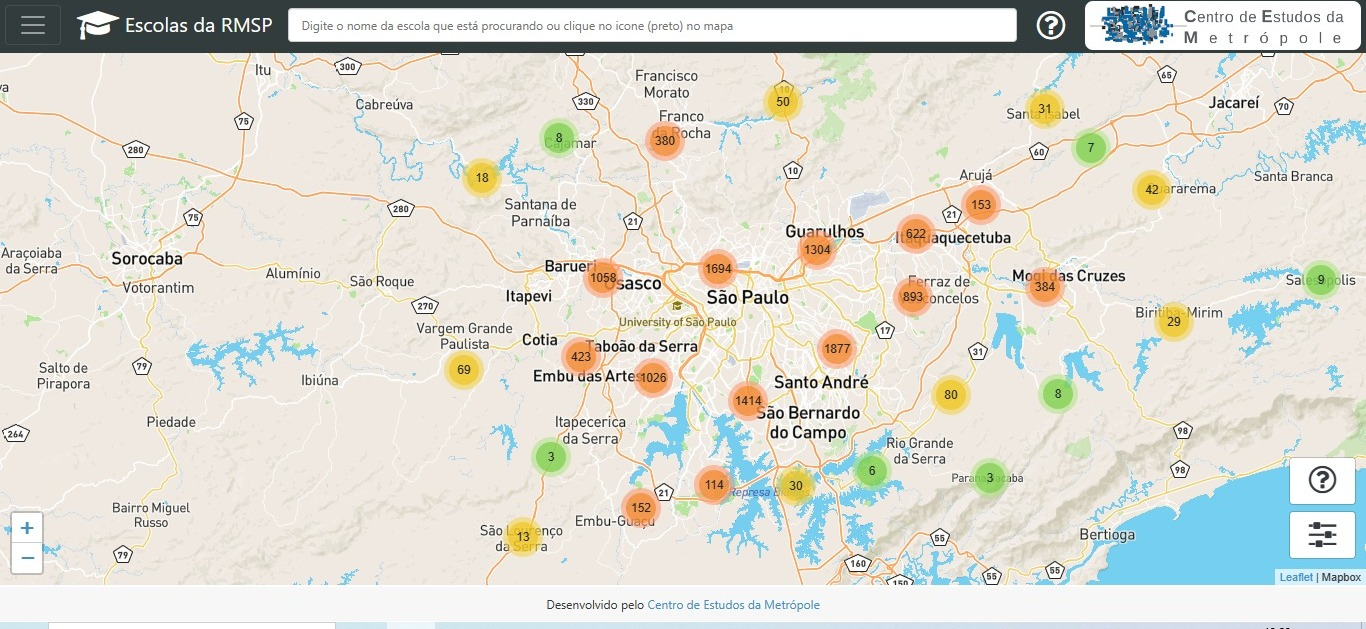
\includegraphics[width=\textwidth]{Figuras/siteCEM.jpeg}
    \caption{Mapa de clusters que mostra a quantidade de escolas em cada região. Ao aproximar o mapa, o usuário consegue ver a localização de cada uma das escolas presentes no banco de dados.}
    \label{fig:siteCEM}
\end{figure}

A segunda base coletada foi a base de dados da \href{https://prefeitura.pbh.gov.br/prodabel}{Prodabel}, empresa de informática e informação da prefeitura de Belo Horizonte. A base de dados foi descoberta por meio da referência 1. É uma base de dados mantida e atualizada mensalmente por 27 empresas públicas e privadas de Belo Horizonte. As empresas têm a responsabilidade de reportar qualquer inconsistência que encontrarem, bem como fornecer novos dados a medida que são adquiridos por ela. É uma base considerada confiável pois é constantemente atualizada e é utilizada por diversos serviços da prefeitura. Um exemplo de serviço que utiliza a base de dados é a distribuição dos alunos da rede pública por meio de georeferenciamento. A base conta com 740.000 endereços na data de coleta. A prefeitura também disponibiliza \href{https://bhmap.pbh.gov.br}{site com um mapa} para vizualização do endereços registrados. O endereço está posicionado em cima do edifício representado. Isso pode gerar erro de alguns metros devido a maioria da APIs colocar o endereço na frente do edifício representado. 

\begin{figure}
    \centering
    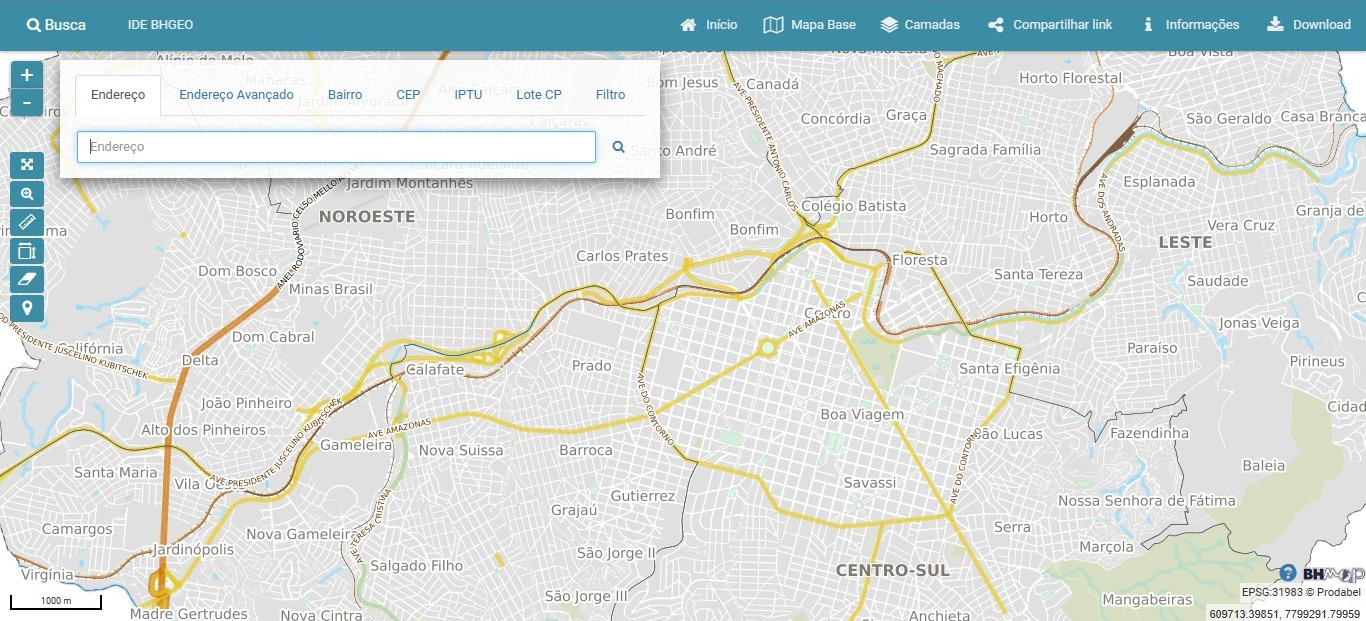
\includegraphics[width=\textwidth]{Figuras/siteProdabel.jpeg}
    \caption{Mapa que mostra a cidade de Belo Horizonte, desenvolvido pela Prodabel. Na barra de pesquisa, é possível pesquisar os endereços e marcá-los no mapa.}
    \label{fig:siteProdabel}
\end{figure}


\section{Processo de Geocodificação}

\begin{figure}
    \centering
    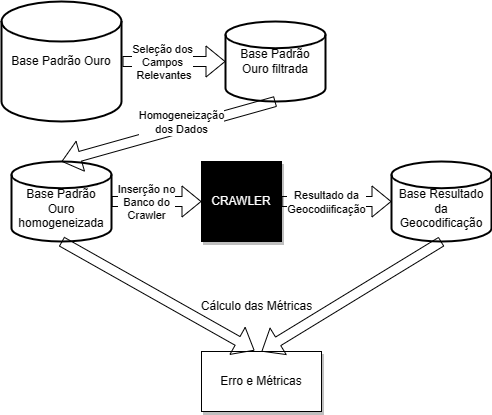
\includegraphics[width=\textwidth]{Figuras/diagrama monografia.drawio.png}
    \caption{Esquematização do processo de preparação e geocodificação dos dados}
    \label{fig:diagramaMono}
\end{figure}

A preparação de dados e geocodificação desempenham um papel crucial em muitos estudos e projetos que envolvem informações geográficas. Nesta pesquisa, esses processos desempenham um papel fundamental na obtenção de dados consistentes e na atribuição de coordenadas geográficas aos endereços.
A etapa de preparação de dados envolve a seleção dos campos relevantes da base de dados, como o nome da rua, número, bairro, CEP e cidade. Além disso, é realizada uma homogeneização dos dados, onde abreviações comumente utilizadas são substituídas por suas formas completas correspondentes. Essa etapa é essencial para garantir resultados mais precisos na geocodificação.
A geocodificação, por sua vez, consiste em atribuir coordenadas geográficas (latitude e longitude) a cada endereço presente na base de dados. Utilizando ferramentas adequadas, o processo de geocodificação é realizado, possibilitando a localização precisa de cada endereço no espaço geográfico.
Para realizar a geocodificação, os endereços previamente preparados são inseridos no banco de dados do Crawler, onde as ferramentas de geocodificação estão disponíveis. Essas ferramentas utilizam algoritmos e informações geográficas para identificar e atribuir as coordenadas geográficas correspondentes a cada endereço. É importante ressaltar que o processo de geocodificação é realizado pela equipe de Back-end do TerraLAB, portanto, vemos esse processo como uma caixa preta.
Uma vez concluída a geocodificação, os endereços geocodificados, juntamente com suas coordenadas geográficas, são armazenados no banco de dados. Esses dados geocodificados podem ser utilizados para análises espaciais, mapeamento e visualização de informações geográficas, contribuindo para a compreensão de padrões e tendências em determinada área de estudo.
Portanto, a preparação de dados e geocodificação são etapas essenciais para garantir a qualidade e a utilidade das informações geográficas utilizadas neste estudo. Esses processos permitem a obtenção de dados consistentes e georreferenciados, facilitando a análise e interpretação dos resultados obtidos

\section{Método de Avaliação}

\subsection{Erro, Acurácia e Discrepância}

A principal métrica utilizada para avaliar a qualidade da geocodificação é o erro do endereço. Esse erro é calculado como a distância entre o ponto de referência e o ponto geocodificado pela GeoAPI. Com base nesse erro, calcularemos medidas estatísticas, como a média, a mediana, o desvio padrão e a média aparada em 5\%, para analisar a precisão das GeoAPIs.

\begin{equation}
    e = D(p_{\text{Gold}}, p_{\text{Geo}})
    \end{equation}
    
    onde:
    \begin{itemize}
      \item $e$ é o erro da geocodificação,
      \item $D$ é uma função que calcula a distância em km,
      \item $p_{\text{Gold}}$ é o ponto da base Gold, e
      \item $p_{\text{Geo}}$ é o ponto resultante da geocodificação.
    \end{itemize}

    
Outra métrica utilizada é a taxa de resposta por API. Para alguns endereços da base de dados, as GeoAPIs podem retornar um erro, não fornecendo uma geocodificação válida. Nesse caso, nada é inserido no banco de dados. A taxa de resposta é calculada como a quantidade de endereços geocodificados dividida pela quantidade de endereços originais na base de dados. Esse valor, normalmente entre 0 e 1, é convertido em uma porcentagem para facilitar a compreensão dos resultados.

\chapter{Resultados} \label{resultado}
Para a primeira etapa do projeto, fizemos a análise do erro e discrepância para os dados de São Paulo. Por problemas na aplicação que coleta as geocodificações, obtivemos resultados apenas para 3 APIs (TomTom, Mapbox e Here). Abaixo serão apresentados os resultados obtidos.

\section{Distribuição Espacial dos Pontos Geocodificados}
Após a geodificação dos dados, era interessante vizualizar como os pontos geocodificados estavam distribuídos no espaço e o quão diferente era dos pontos ouro. Para isso, foram gerados mapas com a identificação dos pontos para cada uma das APIs.

Não é possível tirar muitas conclusões definitivas apenas com essa visualização, no entanto, é possível observar a densidade dos pontos e identificar que em todas as APIs houve uma maior concentração de dados ouro. Porém em algumas APIs essa concentração é visivelmente menor que a outra. Além disso, pode-se notar que os pontos classificados como "Gold" estão concentrados na região metropolitana de São Paulo, enquanto alguns pontos geocodificados estão localizados fora dessa região, em outras cidades do estado. Essa disparidade provavelmente reflete alguns erros graves de geocodificação, conhecidos como outliers.

Na \ref{fig:mapapontos1} podemos vizualizar a distribuição espacial dos pontos geocodificados pela Mapbox. Nela é possível observar a presença dos outliers citados anteriormente. Porém, são poucos os pontos em que houve essa falha. Portanto considerando apenas essa análise, a API teve resultado satisfatório.

\begin{figure}[h]
  \centering
  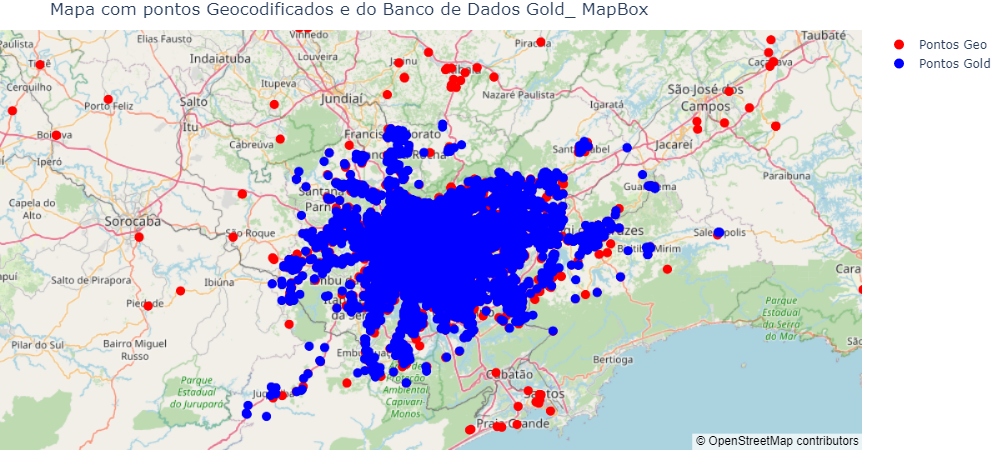
\includegraphics[width=\textwidth]{Figuras/mapapontos1.png}
  \caption{Mapa da Distribuição Espacial dos Pontos da base Gold e Geocodificados pela Mapbox}
  \label{fig:mapapontos1}
\end{figure}

Na \ref{fig:mapapontos2} podemos observar a distribuição espacial dos pontos geocodificados pela Here. Fica claro na imagem que houve uma diminuição significativa dos pontos. O que indica que a resposta da API foi baixa. Com essa quantidade de pontos não é possível tirar conclusões fortes sobre os dados, porém observamos que além da baixa resposta os pontos parecem estar em locais distintos. Esse resultado foi então considerado insatisfatório. Em outro momento, o experimento será repetido para que possamos tirar as conclusões corretas.

\begin{figure}[h]
  \centering
  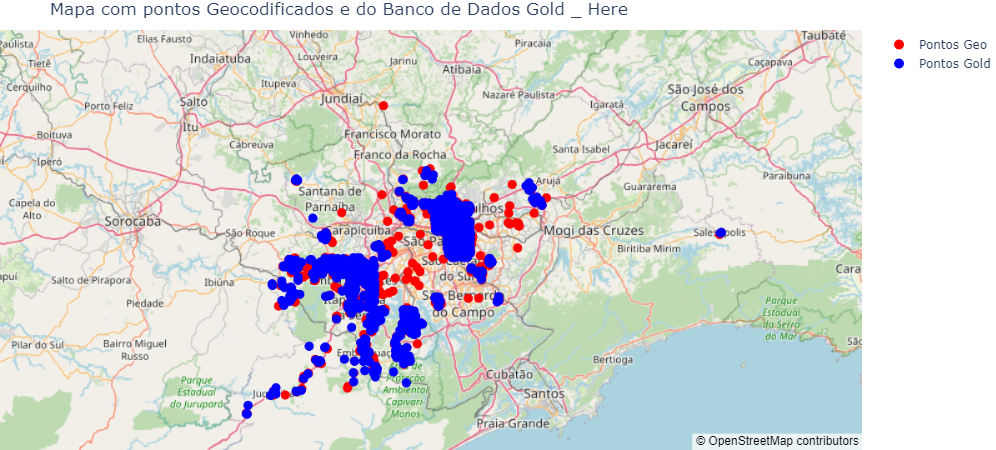
\includegraphics[width=\textwidth]{Figuras/mapapontos2.png}
  \caption{Mapa da Distribuição Espacial dos Pontos da base Gold e Geocodificados pela Here}
  \label{fig:mapapontos2}
\end{figure}

Já a \ref{fig:mapapontos3} mostra a distribuição espacial dos pontos geocodificados pela TomTom. Com esse mapa, é possível observar que a resposta da API foi boa em comparação com os mapas apresentados anteriormente. Também teve alguns outliers e aparentemente esses estão em maior quantidade que na \ref{fig:mapapontos3} e estão mais espaçados geograficamente. Apesar disso, apenas com essa análise, consideramos o resultado satisfatório. 

\begin{figure}[h]
  \centering
  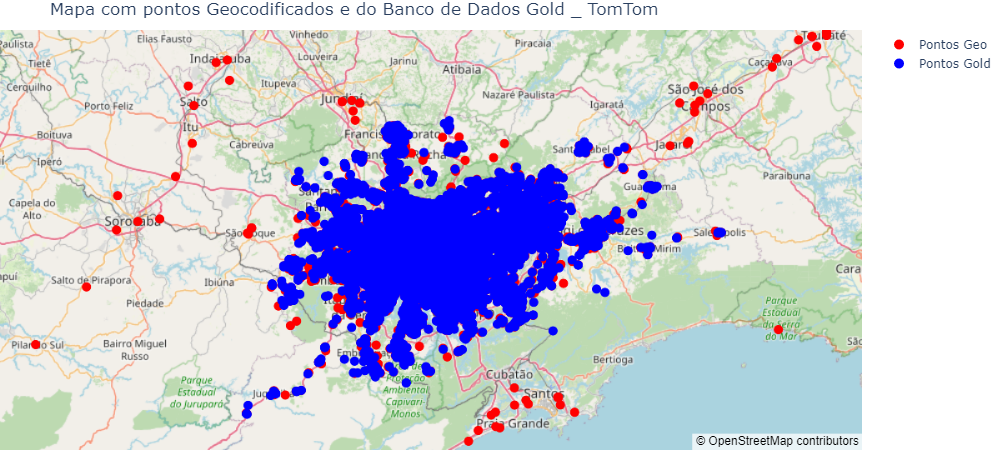
\includegraphics[width=\textwidth]{Figuras/mapapontos3.png}
  \caption{Mapa da Distribuição Espacial dos Pontos da base Gold e Geocodificados pela TomTom}
  \label{fig:mapapontos3}
\end{figure}



\section{Metrícas do Erro}
A próxima etapa foi o calculo do erro para cada um dos pontos, sendo este expresso em quilômetros (Km).

Com o erro de cada um dos pontos, foram calculadas as métricas mencionadas anteriormente. A \ref{tab:tabelaDeMetricas} mostra esses resultados.

Em relação a taxa de resposta, ou seja, a quantidade de endereços que foram geocodificados, a TomTom tem o melhor resultado, com um índice superior a 80\%, seguida pela Mapbox, com taxa de 53,38\%. A Here obteve uma taxa de resposta baixa, como esperado pela análises anteriores. Apesar de ter uma API com taxa de resposta alta, esse resultado foi considerado limitante para equipe pois nos impede de fazer algumas análises.
Outra métrica importante é a taxa de acerto. Foi considerado como acerto aqueles endereços que tiveram erro menor que 150m (0.015Km). A taxa de acerto foi baixíssima para todas as APIs, sendo a melhor 30.19\%. Esse é um resultado péssimo para os dados acumulados. Porém, devido a baixa quantidade de dados não é possível concluir que as APIs em questão tem uma performance ruim. Na próxima etapa do projeto iremos fazer a análise comparativa dos resultados com as outras APIs e com uma maior quantidade de dados. 

Outras métricas interessantes obtidas foram as métricas de média, mediana e desvio padrão. Com elas é possível ver o comportamento geral do erro em cada uma das APIs. As médias foram muito altas, indo de 2Km a 10Km. O desvio padrão também foi alto, mostrando que há uma grande veriação no erro. Apesar disso, a mediana foi bem baixa, alcançando resultados desejáveis na nossa pesquisa. A média aparada obteve resultados muito bons, o que indica que com a retirada dos outliers as métricas tendem a melhorar. Como trabalho futuro, pretendendo refazer as análises com o corte em 50km de erro. De forma geral, esses resultados foram considerados insatisfatórios. Ao longo do relatório, iremos analisar outras questões em detalhes.

\begin{table}
  \centering
  \caption{Métricas de Erro e Resposta}
  \label{tab:tabelaDeMetricas}
  \setlength{\tabcolsep}{4pt}
  \begin{tabular}{|c|c|c|c|c|c|c|}
  \hline
  \makecell{API} & \makecell{Média \\(km)} & \makecell{Mediana \\(km)} & \makecell{Desvio \\Padrão (km)} & \makecell{Média \\Aparada (km)} & \makecell{Taxa de \\Resposta (\%)} & \makecell{Taxa de \\Acerto(\%)}\\
  \hline
  Mapbox & 9.7544 & 0.1084 & 46.7664 & 1.8349 & 53.3829 & 30.1903 \\
  Tomtom & 5.0701 & 0.0560 & 35.6215 & 0.2373 & 83.1894 & 9.2051 \\
  Here & 2.2372 & 0.0632 & 13.7984 & 0.4365 & 13.9075 & 9.2051 \\
  \hline
  \end{tabular}
\end{table}

\subsection{Distribuição do Erro}

Em seguida, foi realizada a análise da distribuição do erro para cada uma das GeoAPIs. 

Para isso, utilizamos histogramas de erro individualmente para cada API e combinando todas elas. Na \ref{fig:hist-global} é mostrado os histogramas para cada uma das APIs e o histograma que é a combinação de todas elas. No entanto, devido à presença de alguns erros exorbitantes, esses histogramas não são muito representativos, pois a maior parte do erro se concentrava entre 0 km e 50 km. O que é considerado um erro muito grande, sendo assim, não se pode tirar conclusões firmes. 

\begin{figure}[ht]
  \centering
  \begin{subfigure}[b]{0.45\textwidth}
    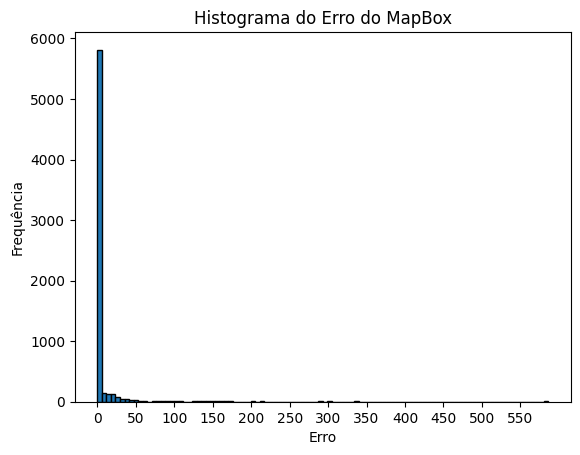
\includegraphics[width=\textwidth]{Figuras/hist1.png}
    \caption{Mapbox}
    \label{fig:hist1}
  \end{subfigure}
  \hfill
  \begin{subfigure}[b]{0.45\textwidth}
    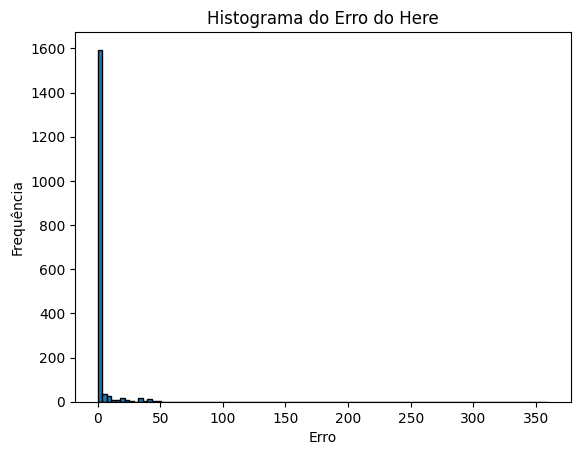
\includegraphics[width=\textwidth]{Figuras/hist2.png}
    \caption{Here}
    \label{fig:hist2}
  \end{subfigure}

  \begin{subfigure}[b]{0.45\textwidth}
    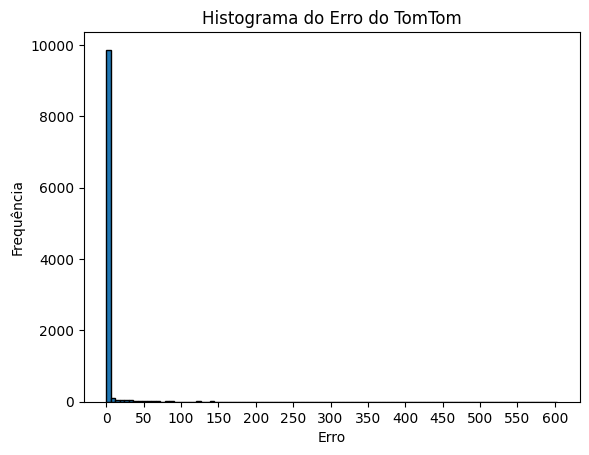
\includegraphics[width=\textwidth]{Figuras/hist3.png}
    \caption{TomTom}
    \label{fig:hist3}
  \end{subfigure}
  \hfill
  \begin{subfigure}[b]{0.45\textwidth}
    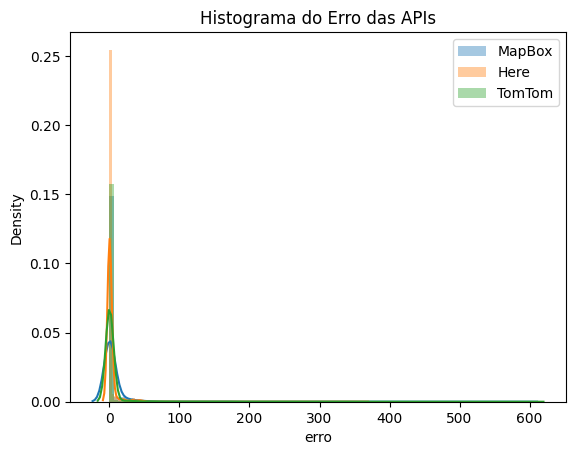
\includegraphics[width=\textwidth]{Figuras/hist4.png}
    \caption{Comparativo entre as APIs}
    \label{fig:hist4}
  \end{subfigure}
  
  \caption{Histogramas do erro das 3 APIs para o todos os dados.}
  \label{fig:hist-global}
\end{figure}

Diante disso, decidimos realizar um corte nos dados, limitando o erro em 0.5 km ou 500 metros. Em seguida, repetimos o processo, agora gerando um único histograma que representa a distribuição do erro para todas as APIs em conjunto. A \ref{fig:histLimitado} apresenta esse histograma. Nele observamos que a maior parte dos dados concentra-se entre erro de 0.0 Km e 0.1 Km. Corroborando assim com a hipótese de que as métricas se comportariam melhor com a retirada dos outliers. Em relação as APIs, nessa faixa de erro a TomTom tem um comportamento melhor, já que a curva está mais estreita e próximo de 0. Poréma diferença entre as APIs não é grande, fazendo com que essa diferença não seja tão significativa. 
 
\begin{figure}[h]
  \centering
  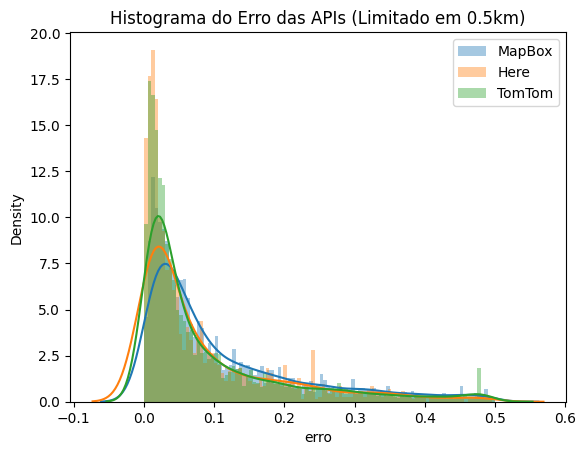
\includegraphics[width=0.8\textwidth]{Figuras/hist5.png}
  \caption{Histograma comparativo do erro das APIs limitado em 500 metros}
  \label{fig:histLimitado}
\end{figure}

De forma geral, apesar do histograma ser uma ferramenta poderosa para análise da distribuição do erro, nesse caso ela não foi tão eficiente por apresentar limitações na presença de valores excessivamente altos. 

\subsection{Distribuição Espacial do Erro}
Além disso, realizamos uma análise adicional para visualizar como esse erro se comporta no espaço. Para isso, criamos mapas de altitude, onde o erro foi utilizado como medida de altitude. Nessa representação, cores mais próximas do vermelho indicam erros mais altos, enquanto cores mais próximas do azul escuro indicam erros mais baixos. Também plotamos os pontos geocodificados no mapa para avaliar a representatividade das cores. Dessa forma, pudemos verificar se uma determinada área apresenta muitos pontos geocodificados ou se há poucos pontos com erros grandes.

Ao analisar os resultados, observamos que a maioria do mapa apresenta erros menores que 34 km, conforme observado nos histogramas acima. No entanto, identificamos alguns pontos com erros grandes, que serão avaliados individualmente posteriormente. É importante ressaltar que encontramos uma limitação devido à presença de erros exorbitantes, ou outliers, o que restringe nossa capacidade de tirar conclusões significativas. Para obter uma melhor compreensão do contraste e da distribuição geográfica do erro, planejamos repetir o experimento realizando um corte em 34 km.

É válido destacar que o mapa é interativo no projeto original, permitindo uma visualização mais detalhada das informações apresentadas.

Na \ref{fig:grafAltM} conseguimos ver a abrangência da geocodificação da Mapbox, ou seja, os pontos geocodificados conseguiram abranger boa parte da região metropolitana de São Paulo. Além disso, o erro ficou concentrado em 25 Km na maior parte do gráfico. Em alguns pontos ela apresentou erros ente 50 km e 100 km, o que já é considerado um ponto preocupante. Existiram alguns erros na faixa de 300 km nas periferias da cidade. Porém, se pode observar que há uma baixíma concentração de pontos, o que indica que existem poucos pontos com erro baixo, que causaram essa vizualização. No centro, existem alguns pontos avermelhados que possuem uma grande concentração de pontos, esse é um dado preocupante pois indica que a API realmente está errando bastante em relação aos dados referência naquela região.

\begin{figure}[h] 
  \centering
  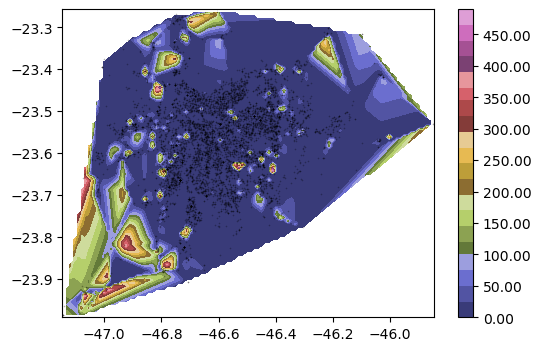
\includegraphics[width=\textwidth]{Figuras/graficoAltPontosMapbox.png}
  \caption{Gráfico de altitude do erro (km) da geocodificação da Mapbox.}
  \label{fig:grafAltM}
\end{figure}

Já a \ref{fig:grafAltH} demostra a baixa abrangência da geocodificação da Here. Como apresentado anteriormente, essa GeoAPI teve a menor texa de resposta e a vizualização pelo gráfico de altitude só confirma isso. Sendo assim, qualquer análise realizada será inviesada. É possível observar uma grande concentração de azul, ou seja, os dados tem erro pequeno. Tem alguns picos, com erro elevado, porém somente um apresenta pontos suficientes para considerar que a região tem erro alto. 

\begin{figure}[h]
  \centering
  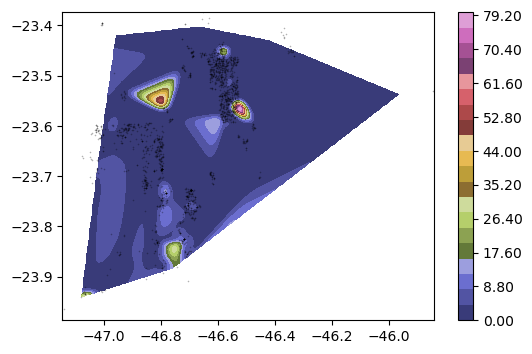
\includegraphics[width=\textwidth]{Figuras/graficoAltPontosHere.png}
  \caption{Gráfico de altitude do erro (km) da geocodificação da Here.}
  \label{fig:grafAltH}
\end{figure}

PAREI AQUI
\begin{figure}[h]
  \centering
  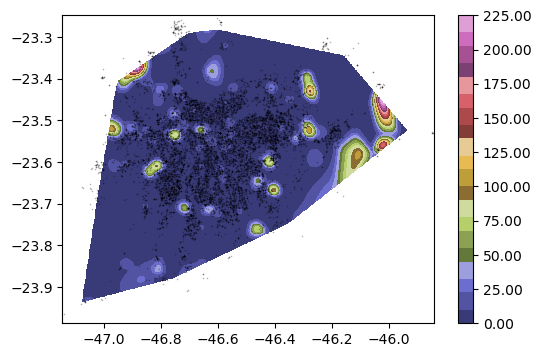
\includegraphics[width=\textwidth]{Figuras/graficoAltPontosTomtom.png}
  \caption{Gráfico de altitude do erro (km) da geocodificação da TomTom.}
  \label{fig:grafAltT}
\end{figure}
\chapter{Considerações Finais} \label{consideracoes}

O presente trabalho apresentou uma análise da qualidade das APIs Mapbox, TomTom e Here para os dados disponibilizados pelo CEM - Centro de estudos da Metrópole. Devido a problemas no Crawler, que é a aplicação que solicita e coleta a geocodificação, tivemos poucas respostas e estas foram insatisfatórias. A conclusão atual é de que as API cometem muitos erros graves e que não há relação clara entre a discrepância e o erro. 

No entanto, quaisquer conclusões tiradas a partir desse estudo são enviesadas a partir do momento em que não temos dados o suficiente e estes são dados específicos. É importante ressaltar que a base de dados possui apenas endereços de escolas, não tendo uma diversidade de imóveis, localizados na região metropolitana de São de Paulo, o que limita a diversidade de localidades consideradas.

Sendo assim, é necessária a repetição do experimento com um maior montante de dados. Para a próxima etapa do trabalho, iremos repetir os experimentos apresentados com uma nova solicitação de geocodificação, além de incluir as APIs faltantes, Google Maps e Open Route Service. Acreditamos que, ao repetir o experimento, possamos compreender melhor o comportamento do erro e comparar os resultados com APIs já consolidadas na academia, como o Google Maps. Além disso, planejamos realizar toda a análise para uma amostra significativa da base de dados da \cite{Prodabel}, que conta com 85 mil endereços distribuídos no espaço. Esperamos que com a maior quantidade de endereços, possamos analisar o comportamento de forma mais clara. Em relação à análise de discrepância, planejamos acrescentar outra medida à análise, a distância para o ponto médio, que acreditamos ser promissora para o trabalho.

Por fim, esclarecemos que o \href{https://chat.openai.com/auth/login?next=%2F}{ChatGPT} foi utilizado durante o trabalho para revisar o texto. O comando "Revise" foi utilizado em textos previamente escritos e depois revisado pelos autores, para garantir a concisão dos dados apresentados. 
 


%% -------------- Elementos Pós-Textuais -----------------%%
\postextual  
\bibliography{bibliografia} % Referências bibliográficas
%%-------------------------------------------------------------
%---------------------- Apêndices ----------------------------
%-------------------------------------------------------------

\begin{apendicesenv}
\partapendices  % Indica o início dos Apendices

\chapter{Diferença entre Anexo e Apêndice}


Os apêndices ``São textos ou documentos elaborados pelo autor, a fim de complementarem sua argumentação, sem prejuízo da unidade nuclear do trabalho'' \cite{NBR14724:2011}. Podem ser incluídos nos apêndices:  os questionários da pesquisas, as tabulação de dados, ilustrações e outros documentos que necessariamente foram preparados pelo autor. Já os anexos, em conformidade com a norma \cite{NBR14724:2011}``são textos ou documentos não elaborados pelo autor, que servem de fundamentação, comprovação ou ilustração à parte do trabalho'', como por exemplo leis, ilustrações, demonstrações de formulas, tabulações de dados de trabalhos referenciados, etc.



\chapter{Formatação}

Os apêndices devem ser identificados por letras maiúsculas consecutivas (APÊNDICE A, APÊNDICE B, etc), travessão e os respectivos títulos, devendo estar
centralizados na folha. 

\end{apendicesenv}

%----------------------------------------------------------------
%---------------------- Anexos ----------------------------------
%----------------------------------------------------------------

\begin{anexosenv}
\partanexos   % indica o início dos anexos
\chapter{Tabelas dos experimentos de formatação completas}
\label{anexo_tabelas_completas}

\section{Resultados Mapbox}

\begin{table}[ht]
\centering
\begin{tabular}{|c|c|c|c|c|c|c|}
\hline
Experimento & Média & Mediana & Desvio & Média & Taxa de & Taxa de \\
 & & & Padrão & Aparada & Resposta & Acerto \\
 & (Km) & (Km) & & (Km) & (\%) & (\%) \\ \hline
1 & 1.539552 & 0.000046 & 10.912322 & 0.511817 & 1.0000 & 0.8506 \\ \hline
1b & 1.855776 & 0.000048 & 9.876150 & 0.826308 & 0.9994 & 0.8088 \\ \hline
2 & 1.985113 & 0.000046 & 12.479481 & 0.880777 & 1.0000 & 0.8246 \\ \hline
2b & 3.747499 & 0.000049 & 26.633204 & 0.712573 & 0.9994 & 0.7982 \\ \hline
3 & 1.660480 & 0.000046 & 11.255071 & 0.578759 & 1.0000 & 0.8400 \\ \hline
3b & 2.268966 & 0.000049 & 13.585637 & 0.831613 & 0.9968 & 0.8056 \\ \hline
4 & 3.239740 & 0.000046 & 33.421642 & 0.579544 & 1.0000 & 0.8466 \\ \hline
4b & 2.395281 & 0.000049 & 18.048547 & 0.618146 & 0.9992 & 0.7986 \\ \hline
5 & 2.270220 & 0.000046 & 25.666232 & 0.597641 & 0.9992 & 0.8380 \\ \hline
5b & 22.718122 & 0.000049 & 151.027338 & 0.722369 & 0.9976 & 0.8100 \\ \hline
\end{tabular}
\caption{Tabela de Resultados para Mapbox para a amostra de Belo Horizonte}
\label{tab:mapboxBH}
\end{table}

\begin{table}[ht]
\centering
\begin{tabular}{|c|c|c|c|c|c|c|}
\hline
Experimento & Média & Mediana & Desvio & Média & Taxa de & Taxa de \\
 & & & Padrão & Aparada & Resposta & Acerto \\
 & (Km) & (Km) & & (Km) & (\%) & (\%) \\ \hline
1 & 9.885009 & 0.264745 & 33.929581 & 5.545753 & 0.9750 & 0.4178 \\ \hline
2 & 13.914447 & 0.481439 & 36.798156 & 8.848430 & 0.9778 & 0.3704 \\ \hline
3 & 12.998989 & 0.287323 & 46.743396 & 6.338832 & 0.9920 & 0.4126 \\ \hline
4 & 9.059893 & 0.287323 & 28.821270 & 5.833966 & 0.9784 & 0.4090 \\ \hline
5 & 13.102779 & 0.287323 & 54.305399 & 6.421116 & 0.9800 & 0.4010 \\ \hline
\end{tabular}
\caption{Tabela de Resultados para MapBox para a amostra de São Paulo}
\label{tab:mapboxSP}
\end{table}
    

\section{Resultados Google}

\begin{table}[ht]
\centering
\begin{tabular}{|c|c|c|c|c|c|c|}
\hline
Experimento & Média & Mediana & Desvio & Média & Taxa de & Taxa de \\
 & & & Padrão & Aparada & Resposta & Acerto \\
 & (Km) & (Km) & & (Km) & (\%) & (\%) \\ \hline
1 & 2.284151 & 0.008843 & 5.067888 & 1.541325 & 0.9992 & 0.7272 \\ \hline
1b & 1.477092 & 0.007045 & 12.541127 & 0.641472 & 0.9996 & 0.8064 \\ \hline
2 & 2.703568 & 0.008981 & 13.275209 & 1.500182 & 0.9998 & 0.7330 \\ \hline
2b & 2.488111 & 0.007888 & 24.657557 & 0.424849 & 0.9984 & 0.7802 \\ \hline
3 & 2.191061 & 0.008868 & 4.905103 & 1.453413 & 0.9992 & 0.7338 \\ \hline
3b & 1.449151 & 0.007442 & 15.764553 & 0.408326 & 1.0000 & 0.7830 \\ \hline
4 & 2.225610 & 0.008894 & 4.911848 & 1.508163 & 0.9990 & 0.7326 \\ \hline
4b & 1.317380 & 0.007442 & 15.783626 & 0.400024 & 0.9992 & 0.7778 \\ \hline
5 & 2.214506 & 0.008916 & 4.911495 & 1.483368 & 0.9992 & 0.7332 \\ \hline
5b & 1.631620 & 0.008843 & 12.503913 & 0.840399 & 0.9988 & 0.7292 \\ \hline
\end{tabular}
\caption{Tabela de Resultados para Google para a amostra de Belo Horizonte}
\label{tab:googleBH}
\end{table}

\begin{table}[ht]
\centering
\begin{tabular}{|c|c|c|c|c|c|c|}
\hline
Experimento & Média & Mediana & Desvio & Média & Taxa de & Taxa de \\
    & & & Padrão & Aparada & Resposta & Acerto \\
    & (Km) & (Km) & & (Km) & (\%) & (\%) \\ \hline
1 & 4.084331 & 0.136854 & 10.741415 & 2.554311 & 0.9988 & 0.5080 \\ \hline
2 & 6.290936 & 0.174920 & 21.319549 & 4.575344 & 0.9986 & 0.4854 \\ \hline
3 & 7.252604 & 0.177119 & 23.235726 & 5.262855 & 0.9988 & 0.4842 \\ \hline
4 & 9.891182 & 0.177119 & 66.380809 & 4.808587 & 0.9988 & 0.4842 \\ \hline
5 & 6.657890 & 0.183598 & 24.621577 & 4.687355 & 0.9990 & 0.4800 \\ \hline
\end{tabular}
\caption{Tabela de Resultados para Google para a amostra de São Paulo}
\label{tab:googleSP}
\end{table}
    

\section{Resultados TomTom}

\begin{table}[ht]
\centering
\begin{tabular}{|c|c|c|c|c|c|c|}
\hline
Experimento & Média & Mediana & Desvio & Média & Taxa de & Taxa de \\
 & & & Padrão & Aparada & Resposta & Acerto \\
 & (Km) & (Km) & & (Km) & (\%) & (\%) \\ \hline
1 & 9.638626 & 0.097375 & 54.293889 & 2.383578 & 1.0000 & 0.5280 \\ \hline
1b & 4.772675 & 0.060837 & 36.194963 & 1.415974 & 0.9998 & 0.5634 \\ \hline
2 & 3.493690 & 0.055936 & 31.276516 & 1.894932 & 0.9994 & 0.5566 \\ \hline
2b & 4.977097 & 0.087184 & 34.512517 & 1.956344 & 0.9998 & 0.5376 \\ \hline
3 & 4.209165 & 0.055609 & 41.653527 & 1.857687 & 1.0000 & 0.5582 \\ \hline
3b & 4.963664 & 0.082551 & 34.529210 & 1.938064 & 0.9988 & 0.5392 \\ \hline
4 & 10.042613 & 0.060228 & 57.575517 & 2.080298 & 0.9998 & 0.5532 \\ \hline
4b & 4.977097 & 0.087184 & 34.512517 & 1.956344 & 0.9998 & 0.5376 \\ \hline
5 & 4.211492 & 0.055581 & 41.665922 & 1.861228 & 0.9994 & 0.5578 \\ \hline
5b & 4.965005 & 0.083011 & 34.522296 & 1.940898 & 0.9992 & 0.5392 \\ \hline
\end{tabular}
\caption{Tabela de Resultados para TomTom para a amostra de Belo Horizonte}
\label{tab:tomtomBH}
\end{table}




\section{Resultados Open Route Service}

\begin{table}[ht]
\centering
\begin{tabular}{|c|c|c|c|c|c|c|}
\hline
Experimento & Média & Mediana & Desvio & Média & Taxa de & Taxa de \\
 & & & Padrão & Aparada & Resposta & Acerto \\
 & (Km) & (Km) & & (Km) & (\%) & (\%) \\ \hline
1 & 5.443245 & 6.606720 & 4.669510 & 5.259343 & 0.9992 & 0.2646 \\ \hline
1b & 134.564517 & 6.726786 & 352.871052 & 70.399993 & 0.9526 & 0.1562 \\ \hline
2 & 141.563530 & 7.689302 & 326.944740 & 85.764655 & 0.9906 & 0.2228 \\ \hline
2b & 235.720433 & 120.745927 & 321.074977 & 190.471249 & 0.9530 & 0.0546 \\ \hline
3 & 215.411691 & 0.450277 & 446.187607 & 148.459274 & 0.9904 & 0.4006 \\ \hline
3b & 221.030496 & 0.545940 & 442.133290 & 155.460776 & 0.9906 & 0.3908 \\ \hline
4 & 7.574040 & 7.585665 & 3.281047 & 7.597740 & 1.0000 & 0.0146 \\ \hline
4b & 152.061311 & 7.894395 & 379.053022 & 86.883669 & 0.9512 & 0.0672 \\ \hline
5 & 7.867047 & 7.587377 & 15.029207 & 7.599037 & 0.9958 & 0.0148 \\ \hline
5b & 5.828340 & 6.606720 & 20.905763 & 5.322782 & 0.9998 & 0.2478 \\ \hline
\end{tabular}
\caption{Tabela de Resultados para Open Route Service para amostra de Belo Horizonte}
\label{tab:orsBH}
\end{table}


\begin{table}[ht]
\centering
\begin{tabular}{|c|c|c|c|c|c|c|}
\hline
Experimento & Média & Mediana & Desvio & Média & Taxa de & Taxa de \\
    & & & Padrão & Aparada & Resposta & Acerto \\
    & (Km) & (Km) & & (Km) & (\%) & (\%) \\ \hline
1 & 8.016763 & 0.346648 & 16.978958 & 6.323177 & 0.9986 & 0.2894 \\ \hline
2 & 149.089363 & 23.343768 & 368.646520 & 80.847362 & 0.9950 & 0.0530 \\ \hline
3 & 22.615834 & 23.022681 & 9.940436 & 22.497670 & 0.9988 & 0.0014 \\ \hline
4 & 111.728383 & 16.604444 & 356.468299 & 45.451290 & 0.9900 & 0.1494 \\ \hline
5 & 19.782864 & 19.499381 & 23.891962 & 18.967053 & 0.9996 & 0.0104 \\ \hline
\end{tabular}
\caption{Tabela de Resultados para OpenRouteService para a amostra de São Paulo}
\label{tab:openrouteserviceSP}
\end{table}
    


\end{anexosenv}

\phantompart  \printindex  % Índice Remissivo
% ----------------------------------------------------------
\end{document}  % fim do documento
